\chapter{Supplementary Results and Artifact Provenance}\chaptermark{Supplementary Results}
\label{chap:appendices}

\section{Secondary RT-DETR metrics}

\begin{table}[htbp]
  \centering
  \caption{Final VIS+IR secondary metrics, mean \(\pm\) sample standard
  deviation over five training checkpoints. COCO mAP averages IoU thresholds
  from 0.50 to 0.95.}
  \label{tab:rtdetr-secondary}
  \begin{adjustbox}{max width=\textwidth}
  \begin{tabular}{lrrrr}
    \toprule
    Configuration & COCO mAP & \mapfifty{} & mAP@75 & mAR@100 \\
    \midrule
    Base & 0.1059 \(\pm\) 0.0243 & 0.3080 \(\pm\) 0.0677 & 0.0474 \(\pm\) 0.0128 & 0.2474 \(\pm\) 0.0302 \\
    FAM & 0.1351 \(\pm\) 0.0096 & 0.3780 \(\pm\) 0.0440 & 0.0692 \(\pm\) 0.0043 & 0.2798 \(\pm\) 0.0141 \\
    FAM + IR Dropout & 0.1360 \(\pm\) 0.0165 & 0.3871 \(\pm\) 0.0469 & 0.0698 \(\pm\) 0.0079 & 0.2764 \(\pm\) 0.0222 \\
    FAM + SSJ & 0.1297 \(\pm\) 0.0095 & 0.3749 \(\pm\) 0.0185 & 0.0625 \(\pm\) 0.0086 & 0.2719 \(\pm\) 0.0331 \\
    Identity DCNv2 & 0.1134 \(\pm\) 0.0305 & 0.3280 \(\pm\) 0.0943 & 0.0560 \(\pm\) 0.0141 & 0.2556 \(\pm\) 0.0357 \\
    Grid Sample & 0.1331 \(\pm\) 0.0077 & 0.3701 \(\pm\) 0.0345 & 0.0631 \(\pm\) 0.0044 & 0.2849 \(\pm\) 0.0115 \\
    \bottomrule
  \end{tabular}
  \end{adjustbox}
\end{table}

\section{Low-threshold qualitative montage}

\begin{figure}[htbp]
  \centering
  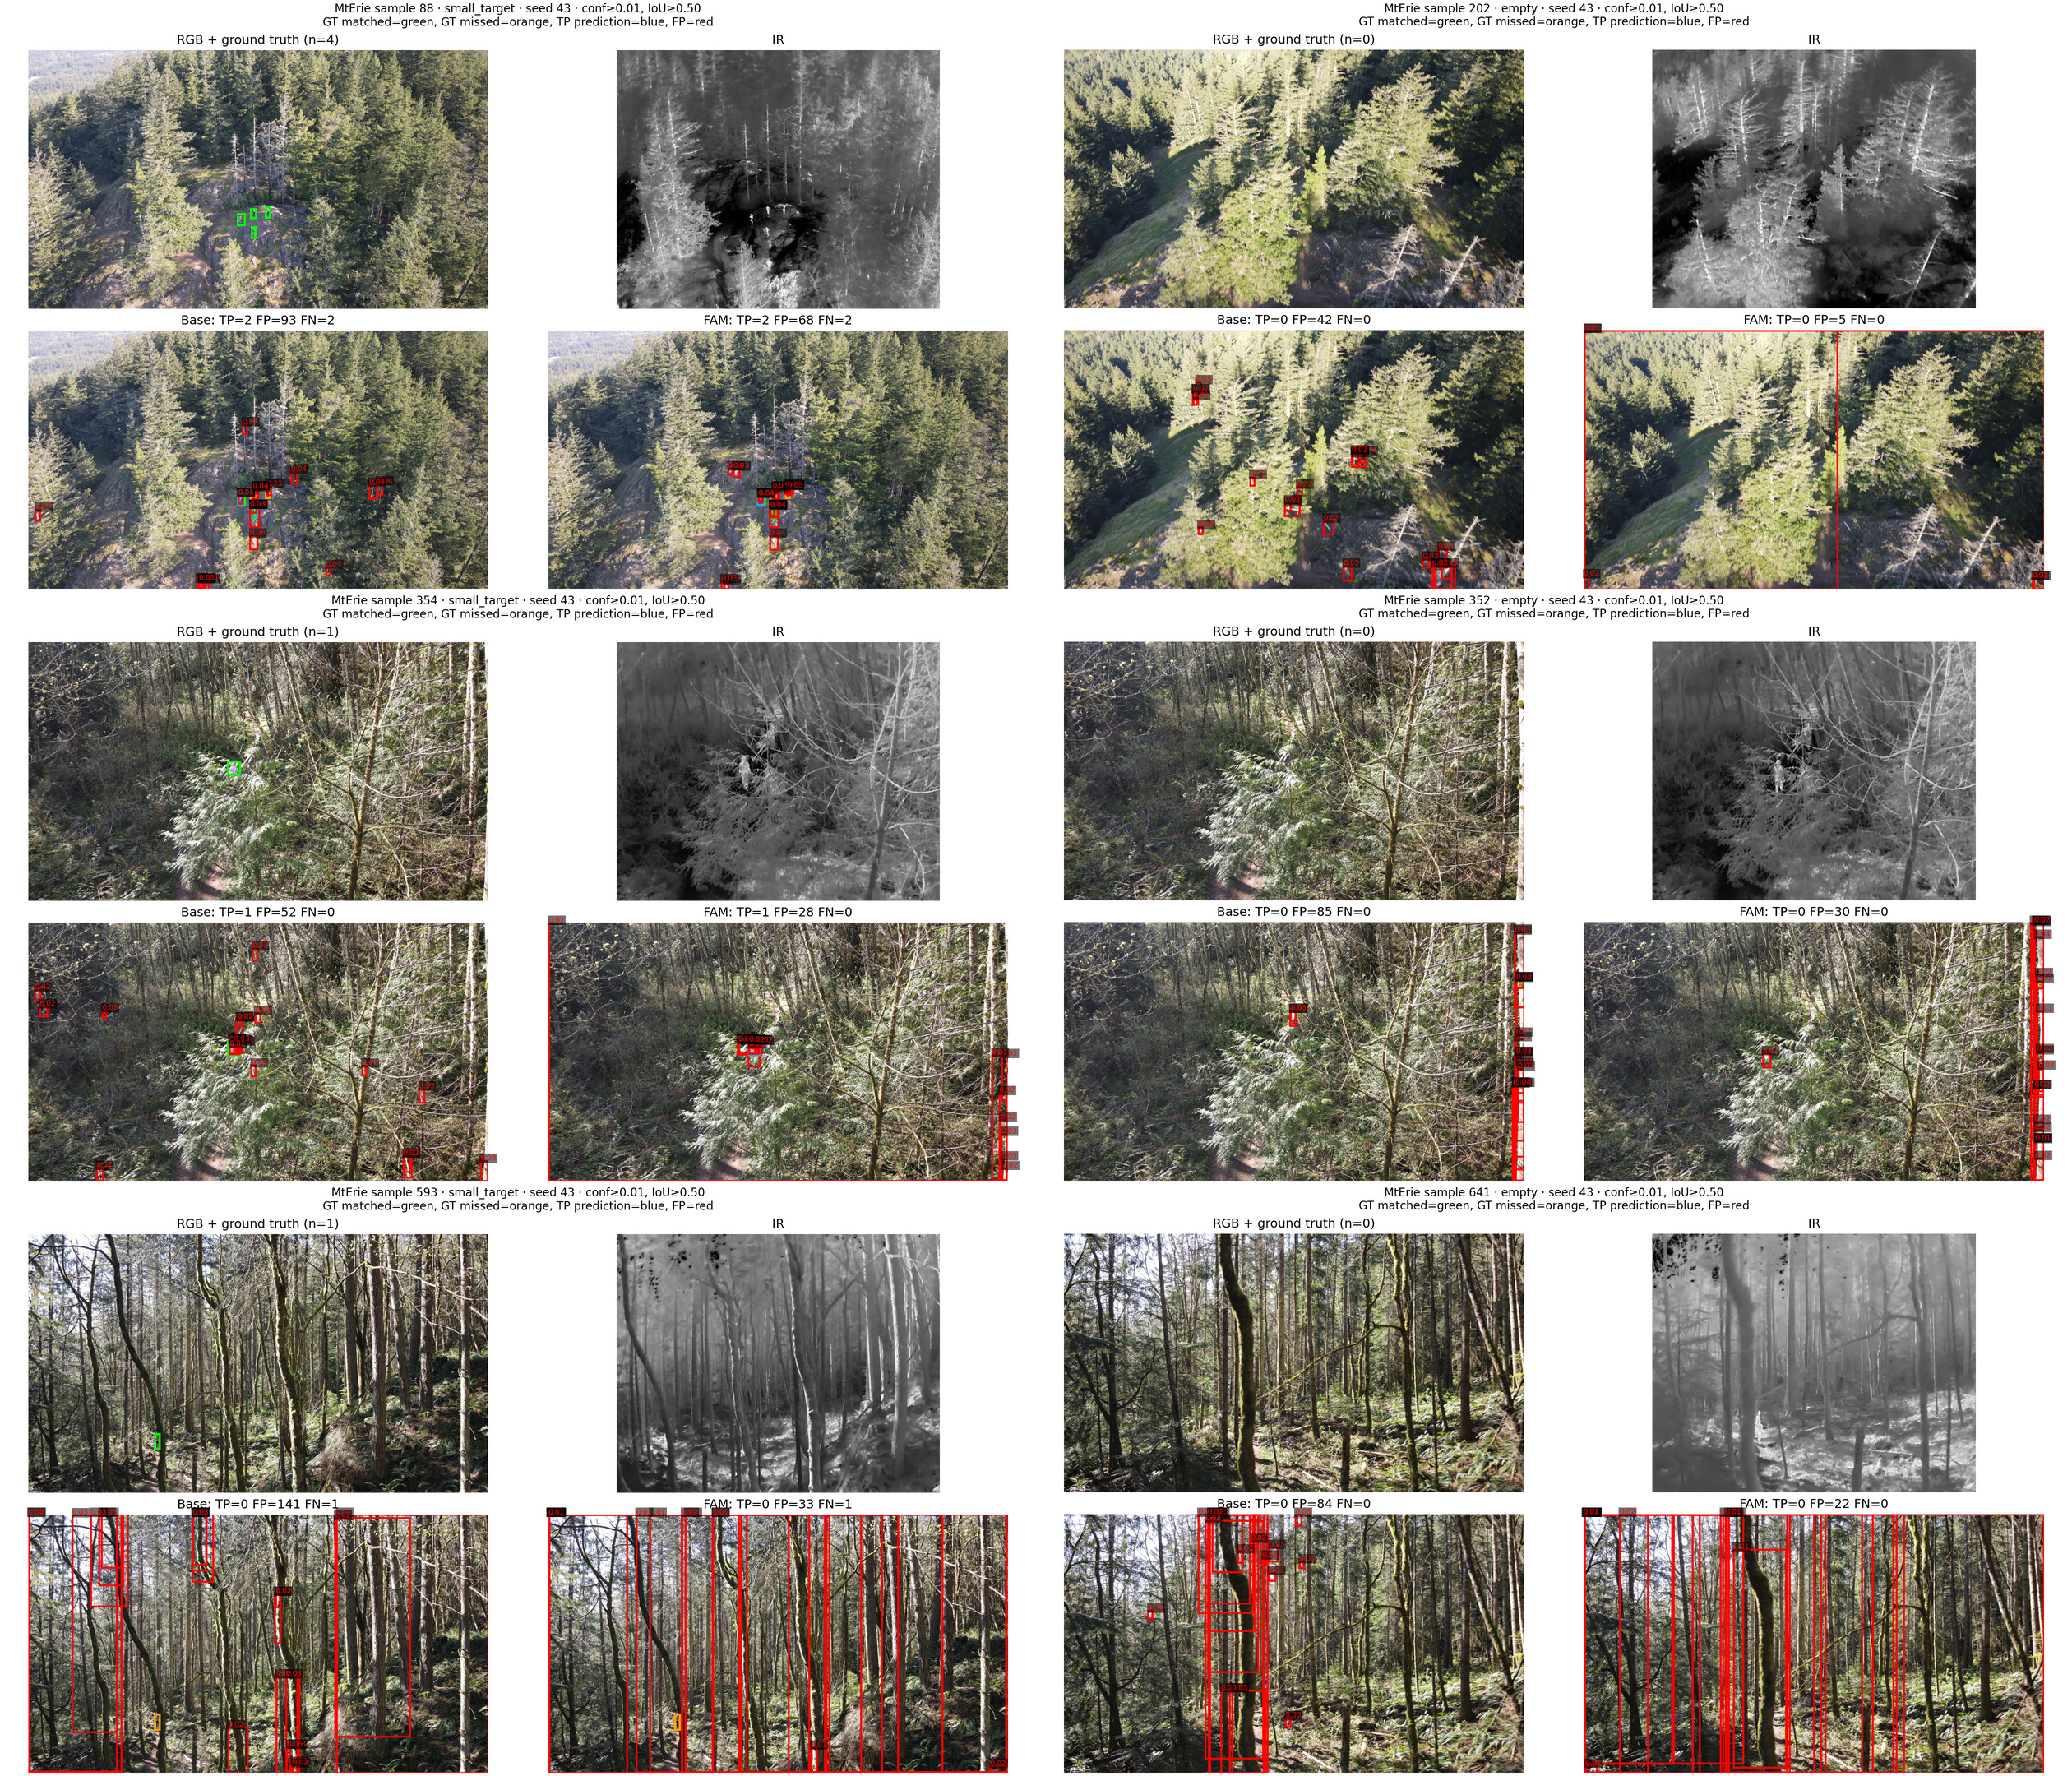
\includegraphics[width=\textwidth]{images/rtdetr_error_qualitative_conf_001.jpg}
  \caption{The six predefined qualitative frames at confidence threshold
  0.01. Titles count all detections, while at most twenty high-score predictions
  are drawn for readability. The density of low-confidence false positives
  illustrates why 0.01 is a metric-collection threshold rather than an
  operational setting.}
  \label{fig:error-qualitative-001}
\end{figure}

\section{Versioned compact artifacts}

Frame-level prediction outputs and diagnostic JSON files are retained in the
local \texttt{out/} directories. The following compact artifacts are stored
with the thesis source:

\begin{longtable}{p{0.38\textwidth}p{0.54\textwidth}}
  \toprule
  Artifact & Content \\
  \midrule
  \endfirsthead
  \toprule
  Artifact & Content \\
  \midrule
  \endhead
  \path{results/rtdetr_error_analysis_checkpoints.csv} & Fifty checkpoint--threshold summaries for Base and FAM on MtErie. \\
  \path{results/rtdetr_carnation_stress_test.csv} & Thirty checkpoint--modality units from the frozen Carnation stress test. \\
  \path{results/rtdetr_compute_benchmark.csv} & Parameter, operation-proxy, latency, throughput, and CUDA-memory summary. \\
  \path{results/rtdetr_fam_sequence_checkpoint_evaluation.csv} & Five-seed Stage-A FAM comparison of validation-selected \texttt{best} and epoch-10 \texttt{latest}. \\
  \path{results/rtdetr_fam_residual_alignment_stage_a_validation.csv} & Paired Stage-A FAM--RCRA validation results. \\
  \path{results/rtdetr_fam_scalar_alignment_control_stage_a_validation.csv} & Three-parameter residual-control attribution results. \\
  \path{results/rtdetr_fam_rcra_full_data_stage_b_evaluation.csv} & Matched full-data FAM--RCRA Stage-B comparison. \\
  \path{results/rtdetr_fam_full_data_paired_modality_evaluation.csv} & Selected-FAM modality interventions on the 708 common paired frames. \\
  \path{results/rtdetr_fam_full_data_native_ir_coordinate_diagnostic.csv} & Post-hoc native-IR coordinate diagnostic on the corresponding 708 IR frames. \\
  \path{results/rtdetr_fam_paired_vis_modal_dropout_probe_evaluation.csv} & Seed-40 Modal Dropout coordinate-system ablation. \\
  \path{results/yolo_final_modality_evaluation.csv} & Thirty final YOLOv10 checkpoint--modality evaluations. \\
  \path{results/rtdetr_unused_acquisition_confirmation.csv} & Fifty frozen evaluations on previously unused internal WiSARD acquisitions. \\
  \path{results/rtdetr_synthetic_geometric_stress.csv} & Six hundred identity and IR-perturbation evaluation points. \\
  \path{results/stage_a_five_seed_comparison.csv} & Thirty-five run records: five seeds each for the FAM reference, mixed consistency, box-guided alignment, and RT-DETRv2/YOLO26 Base and FAM; best and final validation scores. \\
  \path{results/stage_a_five_seed_comparison.json} & Configuration summaries, paired differences, sample deviations, medians, intervals, promotion decisions, and provenance for these Stage-A comparisons. \\
  \path{results/rtdetr_fam_zero_offset_stage_a.csv} & Five paired standard-FAM and zero-offset-initialization records, with best/final validation scores, selection epochs, and replay values. \\
  \path{results/rtdetr_fam_zero_offset_stage_a.json} & Zero-offset initialization protocol, paired summaries, initialization/replay audits, provenance, and Stage-A decision. \\
  \path{images/rtdetr_additive_fam_error_summary.png} & Paired error summary at confidence 0.01. \\
  \path{images/rtdetr_additive_fam_threshold_sensitivity.png} & Multi-threshold error sensitivity analysis. \\
  \path{images/rtdetr_carnation_paired_map50.png} & Carnation paired-seed plot. \\
  \path{images/yolov10_final_modality_paired_map50.png} & Final YOLOv10 paired modality plot. \\
  \path{images/rtdetr_synthetic_geometric_stress_curves.png} & Signed relative-drop curves for controlled IR translation and rescaling. \\
  \path{images/experimental_design.pdf} & Vector diagram of the five-seed experimental design, Stage-A selection, conditional Stage-B confirmation, and separate audits. \\
  \path{images/rtdetr_fam_architecture.pdf} & Vector diagram of the implemented dual-backbone RT-DETR and per-level FAM. \\
  \path{images/rtdetr_final_paired_map50.pdf} & Final paired-seed RT-DETR comparison generated from the primary training outputs. \\
  \path{images/fam_p5_seed41_collapse.png} & Thesis-readable P5 collapse diagnostic assembled from the saved feature diagnostic and JSON statistics. \\
  \path{images/yolov10_dual_backbone_fam.pdf} & Vector diagram of the implemented YOLOv10-s transfer architecture and modality contract. \\
  \bottomrule
\end{longtable}

The artifact README records protocol identifiers, completeness markers, and
checksums of the larger local aggregates. The Stage-A CSV retains per-seed
values and run provenance to make the aggregate tables auditable; these
records are not separate single-run claims. Archived exploratory outputs are
not pooled with the five-seed estimates. The configuration summaries distinguish
live best-selection scores from replay checks and from final-epoch diagnostics.

\section{Code availability}

Model implementations, preprocessing code, experimental configurations, and
analysis scripts are maintained in the project repository. The generated
vector diagrams and comparison figures can be regenerated with
\path{scripts/generate_thesis_figures.py}. Historical public
project material is available at
\url{https://github.com/DonatoFe11/SAR_Fusion}. Checkpoints required for the
reported final diagnostics are preserved locally because model-weight files
were excluded from the experiment tracker uploads.
